\chapter{Poisson 方程式と有限差分法}
\label{chap:poisson-fd}

第1章では、球対称な密度分布を数値積分して重力場を求めた。
本章では、重力ポテンシャルを介して同じ重力場を求める過程を通して、境界値問題の数値解法と数値微分を学ぶ。

基本となる手法は、格子点上の関数値の差を用いて微分を近似する\textbf{有限差分法（finite-difference method）}である。
この考え方は、さまざまな常微分方程式や偏微分方程式に適用できる。
本章で Poisson 方程式を取り上げるのは、離散化、境界条件の組み込み、連立一次方程式の構成、数値解の検証を、解析解の分かる重力モデルで学べるためである。
実際の重力計算法は質量分布の表現や計算の目的によって異なるが\footnote{重力計算法の使い分けは、付録\ref{app:axisym-poisson}の補足「シミュレーション天文学で使う重力計算法」で紹介する。}、ここでは手順を追いやすい有限差分法を用い、1次元の境界値問題として解く。
さらに、得られたポテンシャルから重力加速度を求めるため、前進差分・後退差分・中心差分による\textbf{数値微分（numerical differentiation）}を行い、それぞれの精度を収束試験で比較する。

\begin{learningbox}[本章で学ぶこと]
\begin{itemize}
 \item 球対称 Poisson 方程式を、変数変換 $u=r\Phi$ により有限区間上の1次元境界値問題として設定できる。
 \item 二階微分を中心差分で近似し、中心と外側の境界条件を組み込んだ三重対角の連立一次方程式 $A\boldsymbol{u}=\boldsymbol{b}$ を構成できる。
 \item 前進差分・後退差分・中心差分を Taylor 展開から導き、数値微分に適用できる。
 \item 解析解との比較と格子収束試験から、境界値問題の数値解と数値微分の誤差・収束次数を評価できる。
 \item 連立一次方程式の残差と離散化誤差を区別し、残差が小さくても元の微分方程式に対する誤差が残る理由を説明できる。
\end{itemize}
\end{learningbox}



% =====================================================================
\section{Plummer 球の重力を求める二つの方法}
\label{sec:ch2-plummer}

第1章と同じ Plummer 密度分布
\begin{equation}
 \rho(r)=\frac{3M}{4\pi a^3}\left(1+\frac{r^2}{a^2}\right)^{-5/2}
\label{eq:ch2-plummer-density}
\end{equation}
を使う\cite{ryden2025}。

密度分布から重力ポテンシャル $\Phi$ を求めるには、両者を結ぶ Poisson 方程式
\begin{equation}
 \nabla^2\Phi=4\pi G\rho
\end{equation}
を、適切な境界条件のもとで解く。
球対称系では、得られたポテンシャル $\Phi(r)$ の微分から、重力加速度の動径成分を $g_r(r)=-d\Phi/dr$ と求められる。
ここでは動径方向の外向きを正とする。

Plummer 球では、ポテンシャルと重力加速度の解析式が分かっているため、数値計算の結果を直接検証できる。
無限遠でポテンシャルが0になるように基準を選び、$\Phi(\infty)=0$ とすると、
\begin{equation}
 \Phi_{\rm exact}(r)=-\frac{GM}{\sqrt{r^2+a^2}}
\label{eq:ch2-plummer-potential}
\end{equation}
である。
この式を微分すると、重力加速度は次のように求められる。
\begin{equation}
 g_{r,\rm exact}(r)=-\frac{d\Phi_{\rm exact}}{dr}=-\frac{GMr}{(r^2+a^2)^{3/2}}
\label{eq:ch2-plummer-gravity}
\end{equation}

また、式\eqref{eq:ch1-plummer-mass-exact}で得た内包質量
\begin{equation}
 M(<r)
 =M\frac{(r/a)^3}{[1+(r/a)^2]^{3/2}}
\label{eq:ch2-plummer-mass}
\end{equation}
からも、球対称性を使って
\begin{equation}
 g_r(r)=-\frac{GM(<r)}{r^2}
\label{eq:ch2-gravity-from-mass}
\end{equation}
と求められる。

したがって Plummer 球では、同じ $g_r$ を
\begin{equation}
 \rho\rightarrow M(<r)\rightarrow g_r,
 \qquad
 \rho\rightarrow\Phi\rightarrow g_r
\label{eq:ch2-three-routes}
\end{equation}
という二つの方法で計算でき、それぞれを解析解 $g_{r,\rm exact}$ と比較できる。
同じ物理量を独立した方法で求めて比較することは、数値計算を検証するうえで有用である。
数値積分、Poisson 方程式の求解、数値微分を組み合わせた比較は、Notebook 2 の総合演習で行う。

\begin{notebookblock}{2｜Plummer 球}
Notebook では $G=M=a=1$ の無次元単位を用いる。
密度と内包質量には式\eqref{eq:ch2-plummer-density}、\eqref{eq:ch2-plummer-mass}を、ポテンシャルと重力加速度には式\eqref{eq:ch2-plummer-potential}、\eqref{eq:ch2-plummer-gravity}を使い、検証用の関数として定義する。

{\sffamily\small\color{graytext}対応セル（計算部分）}
\begin{Verbatim}[xleftmargin=2mm,fontsize=\small,frame=single,framesep=1.8mm,framerule=0.35pt,rulecolor=\color{listingframe},fillcolor=\color{listingbg}]
# 無次元単位を設定する
G = 1.0
M = 1.0
a = 1.0

# Plummer 球の密度と解析解
def rho_plummer(r, M, a):
    return 3.0 * M / (4.0 * np.pi * a**3) * (1.0 + (r / a)**2)**(-2.5)

def mass_plummer_exact(r, M, a):
    s = r / a
    return M * s**3 / (1.0 + s**2)**1.5

def phi_plummer_exact(r, G, M, a):
    return -G * M / np.sqrt(r**2 + a**2)

def gravity_plummer_exact(r, G, M, a):
    return -G * M * r / (r**2 + a**2)**1.5
\end{Verbatim}
\end{notebookblock}

% =====================================================================
\section{球対称 Poisson 方程式の1次元化}
\label{sec:ch2-spherical-poisson}

前節で示した Poisson 方程式を球対称系で考える。
球対称なら、密度とポテンシャルは半径 $r$ だけの関数となり、
Poisson 方程式は
\begin{equation}
 \frac{1}{r^2}\frac{d}{dr}
 \left(r^2\frac{d\Phi}{dr}\right)
 =4\pi G\rho(r)
\label{eq:ch2-poisson-spherical}
\end{equation}
と書ける。
したがって、3次元の偏微分方程式は、半径 $r$ だけを独立変数とする二階の常微分方程式へ帰着する。

式\eqref{eq:ch2-poisson-spherical}の左辺を展開すると
\begin{equation}
 \frac{d^2\Phi}{dr^2}
 +\frac{2}{r}\frac{d\Phi}{dr}
 =4\pi G\rho(r)
\end{equation}
である。
この形でも離散化できるが、$r=0$ では $2/r$ の係数をそのまま扱えない。
そこで、球対称 Poisson 方程式をより単純な形にするため、
\begin{equation}
 u(r)\equiv r\Phi(r)
\label{eq:ch2-u-def}
\end{equation}
を導入する。以下、プライムは $r$ に関する微分を表す。
$r>0$ では $\Phi=u/r$ なので、
\begin{align}
 \frac{d\Phi}{dr}
 &=\frac{u'}{r}-\frac{u}{r^2},\\
 r^2\frac{d\Phi}{dr}
 &=ru'-u,\\
 \frac{d}{dr}\left(r^2\frac{d\Phi}{dr}\right)
 &=ru''
\end{align}
となる。
この結果を式\eqref{eq:ch2-poisson-spherical}に代入し、$r>0$ で両辺に $r$ を掛けると、
\begin{equation}
 \frac{d^2u}{dr^2}=4\pi G r\rho(r)
\end{equation}
を得る。
さらに、右辺を
\begin{equation}
 s(r)\equiv4\pi G r\rho(r)
\label{eq:ch2-source-def}
\end{equation}
と書けば、
\begin{equation}
\boxed{
 u''(r)=s(r)
 }
\label{eq:ch2-u-poisson}
\end{equation}
となる。
変数変換 $u=r\Phi$ によって、球対称座標に由来する $1/r$ を含む係数が消え、
左辺は単純な二階微分だけになった。
このため、次節では $u''$ を中心差分で近似することで、内部格子点の方程式を直接構成できる。

式\eqref{eq:ch2-u-poisson}は二階の常微分方程式であり、解を定めるには二つの独立な条件が必要である。
本章では $0\le r\le r_{\max}$ を計算領域とし、その両端で $u$ の値を指定する。
微分方程式に加えて、境界で与えた条件を満たす解を求めることになる。

\begin{definitionbox}{境界値問題}
微分方程式と、計算領域の境界で与える条件を組み合わせて解を求める問題を
\textbf{境界値問題（boundary-value problem）}と呼ぶ。
\end{definitionbox}

中心と外側で具体的に与える境界値は、§\ref{sec:ch2-boundaries}で説明する。

% =====================================================================
\section{Poisson 方程式の中心差分による離散化}
\label{sec:ch2-second-difference}

式\eqref{eq:ch2-u-poisson}では、未知量は半径 $r$ の連続関数 $u(r)$ である。
数値計算では、計算領域を有限個の格子点に分け、
各格子点での関数値を未知数として求める。
そのため、微分方程式に含まれる微分を、
格子点上の有限個の関数値を用いて近似する。

この置き換えによって、連続な微分方程式は、
有限個の未知数に対する代数方程式へ近似的に置き換えられる。
本章で扱う Poisson 方程式は線形なので、
内部格子点で得られる差分方程式と境界条件をまとめると、
連立一次方程式として数値解を求めることができる。
このように、連続な問題を有限個の未知数からなる問題へ置き換えることを
\textbf{離散化（discretization）}という。

ここでは、二階微分 $u''$ を中心差分で近似して、
式\eqref{eq:ch2-u-poisson}を離散化する。
計算領域 $0\le r\le r_{\max}$ を $N$ 個の区間に等分し、
\begin{equation}
 r_i=i\Delta r,
 \qquad
 \Delta r=\frac{r_{\max}}{N},
 \qquad i=0,1,\ldots,N
\label{eq:ch2-grid}
\end{equation}
という等間隔格子を導入する。
格子点は $N+1$ 個である。
滑らかな関数 $u(r)$ の格子点での値を $u_i=u(r_i)$ とし、
$u_i'=u'(r_i)$ などと書く。

内部格子点 $r_i$ のまわりで $u_{i\pm1}=u(r_i\pm\Delta r)$ を Taylor 展開すると、
\begin{align}
 u_{i+1}&=u_i+\Delta r\,u_i'+\frac{(\Delta r)^2}{2}u_i''+\frac{(\Delta r)^3}{6}u_i'''+O((\Delta r)^4),\\
 u_{i-1}&=u_i-\Delta r\,u_i'+\frac{(\Delta r)^2}{2}u_i''-\frac{(\Delta r)^3}{6}u_i'''+O((\Delta r)^4)
\end{align}
である。
2式を足して $2u_i$ を引くと、表示した1次と3次の項が消え、
\begin{equation}
 u_{i+1}-2u_i+u_{i-1}=(\Delta r)^2u_i''+O((\Delta r)^4)
\end{equation}
となる。
両辺を $(\Delta r)^2$ で割ると、
\begin{equation}
 \frac{u_{i+1}-2u_i+u_{i-1}}{(\Delta r)^2}=u_i''+O((\Delta r)^2)
\end{equation}
を得る。
したがって、二階微分は
\begin{equation}
 \boxed{u_i''\simeq\frac{u_{i+1}-2u_i+u_{i-1}}{(\Delta r)^2}}
\label{eq:ch2-second-central}
\end{equation}
と近似できる。
これが二階微分の3点中心差分であり、この近似の打ち切り誤差は $O((\Delta r)^2)$ である。

次に、この中心差分を式\eqref{eq:ch2-u-poisson}へ代入し、
各内部格子点で数値近似が満たす方程式を作る。
ここまでの Taylor 展開では $u_i=u(r_i)$ を厳密な格子点値として用いたが、
以下では記号を簡単にするため、格子点 $r_i$ における数値近似も $u_i$ と書く。
また、既知の右辺を $s_i=s(r_i)$ とする。
各内部格子点では
\begin{equation}
 \frac{u_{i+1}-2u_i+u_{i-1}}{(\Delta r)^2}=s_i
\end{equation}
となる。
後で係数行列の対角成分を正に書くため、両辺に $-(\Delta r)^2$ を掛けると、
\begin{equation}
 \boxed{
 -u_{i-1}+2u_i-u_{i+1}
 =-(\Delta r)^2s_i
 }
\label{eq:ch2-discrete-poisson}
\end{equation}
を得る。

ここで、差分公式がどの格子点を使っているかを整理しておく。

\begin{definitionbox}{差分ステンシル}
ある格子点の差分式を構成するために用いる格子点の組を、
\textbf{差分ステンシル（finite-difference stencil）}と呼ぶ。
本節の二階中心差分では $r_{i-1},r_i,r_{i+1}$ の3点を使うため、
式\eqref{eq:ch2-discrete-poisson}は3点ステンシルである
（図\ref{fig:ch2-stencil}）。
\end{definitionbox}

\begin{figure}[!htbp]
\centering
\begin{tikzpicture}[>=Latex,font=\sffamily\small]
 \node[anchor=east,text=navy] at (-0.15,1.18) {Coefficient};
 \node[anchor=east] at (-0.15,0.64) {Unknown};
 \node[anchor=east] at (-0.15,-0.28) {Grid point};
 \draw[thick] (0.7,0)--(8.3,0);
 \foreach \x/\rlab/\ulab/\coef in {1.2/{r_{i-1}}/{u_{i-1}}/{-1},4.5/{r_i}/{u_i}/{+2},7.8/{r_{i+1}}/{u_{i+1}}/{-1}}{
   \filldraw[fill=white,line width=0.7pt] (\x,0) circle (2.5pt);
   \node at (\x,-0.28) {$\rlab$};
   \node at (\x,0.64) {$\ulab$};
   \node[text=navy,font=\large] at (\x,1.18) {$\coef$};
 }
 \draw[<->,gray] (1.2,-0.76)--node[below]{$\Delta r$}(4.5,-0.76);
 \draw[<->,gray] (4.5,-0.76)--node[below]{$\Delta r$}(7.8,-0.76);
\end{tikzpicture}
\caption{式\eqref{eq:ch2-discrete-poisson}の3点ステンシル。上段は左辺における $u_{i-1},u_i,u_{i+1}$ の係数である。二階微分の中心差分そのものの係数 $1,-2,1$ ではなく、式\eqref{eq:ch2-discrete-poisson}で用いる係数 $-1,2,-1$ を示している。}
\label{fig:ch2-stencil}
\end{figure}

% =====================================================================

\section{中心と外側の境界条件}
\label{sec:ch2-boundaries}

前節で得た内部格子点の差分式に加えて、計算領域の両端で境界条件を与える。
本章では $0\le r\le r_{\max}$ で式\eqref{eq:ch2-u-poisson}を解くため、中心 $r=0$ と外側 $r=r_{\max}$ の値を指定する。

\subsection{中心境界条件と $\Phi(0)$ の復元}

中心でポテンシャル $\Phi(0)$ が有限なら、
$u=r\Phi$ なので
\begin{equation}
 u(0)=0
\label{eq:ch2-u0}
\end{equation}
である。
したがって、$u$ について Poisson 方程式を解くときの中心境界条件は
\begin{equation}
 u_0=0
\end{equation}
と与えればよい。

一方、Poisson 方程式を解いた後で $u$ からポテンシャル $\Phi$ を復元するときには、
中心だけ別の扱いが必要になる。
$r_i>0$ では
\begin{equation}
 \Phi_i=\frac{u_i}{r_i}
\end{equation}
とすればよいが、中心では $u_0=r_0=0$ なので、
この式は $0/0$ となり直接使えない。
これは $u$ の中心境界条件に問題があるのではなく、
変数変換 $u=r\Phi$ から $\Phi$ に戻すときに生じるものである。

中心でポテンシャルが滑らかなら
\begin{equation}
 \Phi(0)
 =\lim_{r\to0}\frac{u(r)}{r}
 =u'(0)
\label{eq:ch2-center-limit}
\end{equation}
である。
この滑らかさと球対称性による中心まわりの対称性を用いると、
中心値 $\Phi_0=\Phi(0)$ は中心近傍の2点から
\begin{equation}
 \boxed{
 \Phi_0
 \simeq
 \frac{4\Phi_1-\Phi_2}{3}
 }
\label{eq:ch2-center-phi}
\end{equation}
と近似できる（「補足｜中心ポテンシャルの外挿公式の導出」を参照）。
実際に Poisson 方程式で求める未知数は $u$ なので、
$\Phi_1=u_1/\Delta r$、
$\Phi_2=u_2/(2\Delta r)$ を代入すると
\begin{equation}
 \boxed{
 \Phi_0
 \simeq
 \frac{8u_1-u_2}{6\Delta r}
 }
\label{eq:ch2-center-u}
\end{equation}
となる。数値計算では、この式を用いて中心ポテンシャルを復元する。

\begin{topicblock}{中心ポテンシャルの外挿公式の導出}
中心を通る任意の直線上に、中心を $\ell=0$ とする符号付き座標 $\ell$ を取る。
球対称性から、中心から同じ距離にある $\ell$ と $-\ell$ では
ポテンシャルが等しいので、
\begin{equation}
 \Phi(\ell)=\Phi(-\ell)
\end{equation}
が成り立つ。
中心で $\Phi$ が滑らかなら $\Phi$ は $\ell$ の偶関数であり、
中心まわりの Taylor 展開には偶数次の項だけが現れる。
半径 $r=|\ell|$ を用いると
\begin{equation}
 \Phi(r)=\Phi_0+c_2r^2+c_4r^4+O(r^6)
\end{equation}
と書ける。

$r_1=\Delta r$、$r_2=2\Delta r$ とすると
\begin{align}
 \Phi_1&=\Phi_0+c_2(\Delta r)^2+c_4(\Delta r)^4+O((\Delta r)^6),\\
 \Phi_2&=\Phi_0+4c_2(\Delta r)^2+16c_4(\Delta r)^4+O((\Delta r)^6).
\end{align}
ここで $4\Phi_1-\Phi_2$ を作ると $(\Delta r)^2$ の項が消え、
\begin{equation}
 \frac{4\Phi_1-\Phi_2}{3}
 =\Phi_0-4c_4(\Delta r)^4+O((\Delta r)^6)
\end{equation}
となる。
したがって、
\begin{equation}
 \Phi_0
 =\frac{4\Phi_1-\Phi_2}{3}
 +O((\Delta r)^4)
\end{equation}
を得る。
さらに
$\Phi_1=u_1/\Delta r$、
$\Phi_2=u_2/(2\Delta r)$ を代入すると、
式\eqref{eq:ch2-center-u}が得られる。

ただし、この $O((\Delta r)^4)$ は、
$\Phi_1,\Phi_2$ が厳密に分かっている場合の外挿誤差である。
実際には、これらも有限差分法で求めた近似値であり、
誤差を含むため、中心ポテンシャルが4次精度で求まるとは限らない。
\end{topicblock}


\subsection{外側境界条件}

もう一つの境界条件は、計算領域の外側 $r=r_{\max}$ に与える。
まず有限差分法そのものの精度を検証するため、
本章の Plummer 球では解析解を用いて
\begin{equation}
 u_N
 =r_{\max}\Phi_{\rm exact}(r_{\max})
\label{eq:ch2-outer-exact}
\end{equation}
とする。
これにより、外側境界の近似による誤差を入れずに、
主として有限差分による離散化誤差を調べることができる。

解析解が分からなくても、全質量 $M$ が有限な孤立系では、
十分遠方で質量分布を点質量として近似し、
\begin{equation}
 \Phi(r)\simeq-\frac{GM}{r},
 \qquad
 u(r)\simeq-GM
\label{eq:ch2-outer-pointmass}
\end{equation}
を外側境界条件として用いることができる。
ただし、本章の Plummer 球は $r_{\max}$ より外側にも広がっているため、
有限の $r_{\max}$ でこの近似を境界値に用いると、解析値との差が生じる。
この誤差は有限差分の離散化誤差とは別のものであり、
$r_{\max}$ を十分大きく取るか、より適切な外側境界条件を用いることで小さくする必要がある。
この影響は Notebook 2 の発展課題「境界条件による誤差」で調べる。

本章では、有限の計算領域で Poisson 方程式を解くために、外側境界でポテンシャルの値を与えた。
自己重力を含む数値シミュレーションでも、密度分布から重力ポテンシャルを
有限の計算領域上で求める場合には、外側境界条件を指定する必要がある\footnote{
質量分布が境界より十分内側に収まる場合には、点質量による項を先頭とし、非球対称な分布の効果を高次の項で表す
\textbf{多重極展開（multipole expansion）}を用いることがある\cite{tomisaka2007}。
これは質量配置の近似を改良する方法であり、境界より外側の質量を無視したことによる誤差とは区別する。
}。


\begin{topicblock}{孤立系の境界条件と James 法}
本章では Plummer 球の解析解が分かるため、外側境界のポテンシャルを直接与えられる。
一方、一般の非球対称な質量分布では、有限の計算領域の境界上で
どのようなポテンシャルを与えるかが問題になる。
孤立系では無限遠で $\Phi\to0$ となるが、
有限の距離にある境界で単に $\Phi=0$ としても、一般には正しい解にならない。

James 法（James 1977）は、孤立系の境界条件を有限の計算領域で扱う方法である\cite{james1977,bt2008}。
まず、境界上でポテンシャルを0と仮定して Poisson 方程式を解く。
しかし、この仮定は実際の孤立系の境界条件とは異なる。
そこで、境界を0としたことで生じる影響を計算して取り除き、
孤立系に対応するポテンシャルを求める。

James 法は有限差分法を置き換えるものではなく、
Poisson 方程式の数値解法と組み合わせて境界条件を扱う方法である。
ただし、計算領域の外側にも質量がある場合は、その寄与を別途考慮する必要がある。
\end{topicblock}

% =====================================================================
\section{連立一次方程式の組み立て}
\label{sec:ch2-matrix}

式\eqref{eq:ch2-discrete-poisson}には、格子点 $r_i$ における
$u_i$ だけでなく、隣の格子点の値 $u_{i-1}$ と $u_{i+1}$ も含まれる。
したがって、各 $u_i$ を独立に求めることはできず、
すべての内部格子点の差分式をまとめて連立一次方程式として解く必要がある。

まず、差分式がどのような連立一次方程式になるかを見るため、
$r_0,r_1,r_2,r_3,r_4$ の5個の格子点だけを持つ簡単な例を考える。
両端の $r_0,r_4$ は境界点であり、$r_1,r_2,r_3$ は内部格子点である。
この例では、左境界に隣接する $r_1$、両隣が内部点である $r_2$、
右境界に隣接する $r_3$ の3種類の差分式を確認できる。

この例では、両端の $u_0$ と $u_4$ は境界条件によって与えられる。
したがって、求める未知数は内部3点の
\begin{equation}
 u_1,\quad u_2,\quad u_3
\end{equation}
である。
式\eqref{eq:ch2-discrete-poisson}を
$r_1,r_2,r_3$ にそれぞれ適用すると、
\begin{align}
 2u_1-u_2
 &=-(\Delta r)^2s_1+u_0,\\
 -u_1+2u_2-u_3
 &=-(\Delta r)^2s_2,\\
 -u_2+2u_3
 &=-(\Delta r)^2s_3+u_4.
\end{align}
これら3本の式をまとめると、
\begin{equation}
 \begin{pmatrix}
 2&-1&0\\
 -1&2&-1\\
 0&-1&2
 \end{pmatrix}
 \begin{pmatrix}u_1\\u_2\\u_3\end{pmatrix}
 =
 \begin{pmatrix}
 -(\Delta r)^2s_1+u_0\\
 -(\Delta r)^2s_2\\
 -(\Delta r)^2s_3+u_4
 \end{pmatrix}
\label{eq:ch2-small-matrix}
\end{equation}
となる。

ここで、左端の行列を係数行列 $A$、
内部格子点の未知数を並べた列ベクトルを $\boldsymbol{u}$、
既知の量をまとめた右辺の列ベクトルを $\boldsymbol{b}$ と書くと、
式\eqref{eq:ch2-small-matrix}は
\begin{equation}
 A\boldsymbol{u}=\boldsymbol{b}
\label{eq:ch2-linear-system}
\end{equation}
と簡潔に表せる。
一般の $N$ では、
\begin{equation}
 \boldsymbol{u}
 =
 \begin{pmatrix}
 u_1&u_2&\cdots&u_{N-1}
 \end{pmatrix}^{\mathsf T}
\end{equation}
が求める未知数ベクトルである。上付きの $\mathsf{T}$ は転置を表し、横に並べた成分を列ベクトルにしている。
係数行列 $A$ の非零成分は、主対角とその上下の対角にだけ現れる。
このような行列を
\textbf{三重対角行列（tridiagonal matrix）}と呼ぶ。

Listing 2.1 に、一般の $N$ に対して
係数行列 $A$ と右辺ベクトル $\boldsymbol{b}$ を組み立てる部分を示す。

\begin{listingbox}{2.1　三重対角行列と境界値の組み込み}
\begin{Verbatim}[fontsize=\small]
# 内部格子点の値 u_1, ..., u_{N-1} を未知数とする
n = N - 1
A = np.zeros((n, n))

# 三重対角行列の係数 (-1, 2, -1) を入れる
np.fill_diagonal(A, 2.0)
np.fill_diagonal(A[1:], -1.0)
np.fill_diagonal(A[:, 1:], -1.0)

# 内部格子点に対応する右辺ベクトルを作る
b = -(dr**2) * source[1:N].copy()

# 既知の境界値 u_0, u_N を右辺へ組み込む
b[0] += u0
b[-1] += uN
\end{Verbatim}
\end{listingbox}

一般の格子では、未知数は $u_1,\ldots,u_{N-1}$ の $N-1$ 個である。
コード中の \texttt{n = N - 1} はこの未知数の数を表す。
また、\texttt{dr} は格子幅 $\Delta r$、
\texttt{source[1:N]} は内部格子点の
$s_1,\ldots,s_{N-1}$ を取り出している。
係数行列 $A$ の主対角の $2$ と上下の副対角の $-1$ は、
式\eqref{eq:ch2-discrete-poisson}の左辺の係数に対応する。

5格子点の例と同様に、一般の $N$ 区間でも、
両端の境界値 $u_0$ と $u_N$ は未知数に含めず、右辺に組み込む。
コード中の \texttt{b[0] += u0} は、
最初の内部格子点 $r_1$ の式に中心境界値 $u_0$ を加える操作に対応する。
同様に、\texttt{b[-1] += uN} は、
最後の内部格子点 $r_{N-1}$ の式に外側境界値 $u_N$ を加える操作である。
本章では $u_0=0$ なので最初の加算は値を変えないが、
差分式とコードの対応を明示するために残している。


% =====================================================================

\section{Plummer 球の Poisson 方程式の数値解}
\label{sec:ch2-solve-plummer}

ここまで、球対称 Poisson 方程式を有限差分法で解くために、
球対称性による1次元化と変数変換、中心差分による離散化、境界条件の設定、
連立一次方程式の組み立てを順に説明してきた。
本節では、これらの手順をまとめて Plummer 球に適用し、
重力ポテンシャルを数値的に求める。

\medskip
\noindent\textbf{計算手順｜球対称 Poisson 方程式を有限差分で解く}
\par\smallskip
\begin{enumerate}[itemsep=0em,topsep=0.1em]
 \item $r_i=i\Delta r$ の格子を作り、密度 $\rho_i=\rho(r_i)$ と
       右辺 $s_i=4\pi G r_i\rho_i$ を計算する。
 \item 中心境界 $u_0=0$ と外側境界 $u_N$ を与える。
 \item 内部格子点の差分式から、係数行列 $A$ と
       右辺ベクトル $\boldsymbol{b}$ を組み立てる。
 \item 連立一次方程式 $A\boldsymbol{u}=\boldsymbol{b}$ を解き、
       $u_1,\ldots,u_{N-1}$ を求める。
 \item 境界値と内部の数値解を合わせて $u_i$ を構成し、
       $r_i>0$ では $\Phi_i=u_i/r_i$ とする。
       中心値 $\Phi_0$ は式\eqref{eq:ch2-center-u}から復元する。
\end{enumerate}
\medskip

以下では、この一連の手順を Python で実行する。
連立一次方程式の求解には、NumPy の \texttt{np.linalg.solve} を使う。\footnote{一般の密行列には Gauss の消去法や LU 分解が用いられる。本章のような三重対角行列では、構造を利用した Thomas 法によって計算量を $O(N)$ にできる。これらの解法の基本的な考え方は付録\ref{app:linear-systems}、詳しい説明は幸谷 第7章\cite{kouya2021}を参照。}

得られた数値解を検証するため、
ポテンシャルを同じ格子点で評価した解析解と比較する。
あわせて、連立一次方程式をどの程度満たしているかを残差で確認する。

\begin{definitionbox}{残差}
連立一次方程式 $A\boldsymbol{u}=\boldsymbol{b}$ に数値解を代入したときの左右のずれ
\begin{equation}
 \boldsymbol{r}_{\rm res}
 =A\boldsymbol{u}-\boldsymbol{b}
\label{eq:ch2-residual}
\end{equation}
を\textbf{残差（residual）}という。
残差は、数値解が離散化した連立一次方程式をどの程度満たしているかを表す。
残差が小さくても、解析解との誤差が小さいとは限らない。
\end{definitionbox}

\begin{notebookblock}{2｜Poisson 方程式の数値解}
Notebook では、一連の計算手順を関数
\texttt{solve\_\allowbreak spherical\_\allowbreak poisson\_\allowbreak plummer} にまとめる。
関数の内部では、格子と右辺の作成、境界条件の設定、
連立一次方程式の組み立てと求解、$u$ から $\Phi$ への復元を順に行う。
外側境界は引数 \texttt{boundary} で選び、
本節では式\eqref{eq:ch2-outer-exact}の解析的な境界条件を用いる。

{\sffamily\small\color{graytext}対応セル（関数定義）}
\begin{Verbatim}[xleftmargin=2mm,fontsize=\small,frame=single,framesep=1.8mm,framerule=0.35pt,rulecolor=\color{listingframe},fillcolor=\color{listingbg}]
def solve_spherical_poisson_plummer(N, r_max, G, M, a, boundary="exact"):
    # 1. 格子を作り、密度と Poisson 方程式の右辺を計算する
    r = np.linspace(0.0, r_max, N + 1)
    dr = r[1] - r[0]
    rho = rho_plummer(r, M, a)
    source = 4.0 * np.pi * G * r * rho

    # 2. 中心境界と外側境界を与える
    u0 = 0.0
    if boundary == "exact":
        uN = r_max * phi_plummer_exact(r_max, G, M, a)
    elif boundary == "point_mass":
        uN = -G * M
    else:
        raise ValueError("boundary は 'exact' または 'point_mass' を指定")

    # 3. 係数行列 A と右辺ベクトル b を組み立てる
    n = N - 1
    A = np.zeros((n, n))
    np.fill_diagonal(A, 2.0)
    np.fill_diagonal(A[1:], -1.0)
    np.fill_diagonal(A[:, 1:], -1.0)

    b = -(dr**2) * source[1:N].copy()
    b[0] += u0
    b[-1] += uN

    # 4. A u = b を解き、境界値と内部解を合わせる
    u = np.empty(N + 1)
    u[0] = u0
    u[1:N] = np.linalg.solve(A, b)
    u[N] = uN

    # 5. u = r Phi からポテンシャルを復元する
    phi = np.empty(N + 1)
    phi[1:] = u[1:] / r[1:]
    phi[0] = (8.0 * u[1] - u[2]) / (6.0 * dr)

    return r, rho, u, phi, A, b
\end{Verbatim}

この関数が返す配列 \texttt{u} は、両端の境界値を含む $N+1$ 個の値からなる。
連立一次方程式の未知数ベクトル $\boldsymbol{u}$ に対応するのは、内部の $N-1$ 個を取り出した \texttt{u[1:N]} である。
この関数を $N=200$、$r_{\max}=10a$ で実行すると、$\Delta r=0.05a$ となる。
以下では、数値ポテンシャルの最大絶対誤差と、
残差の各成分の絶対値の最大値を計算する。

{\sffamily\small\color{graytext}対応セル（計算部分）}
\begin{Verbatim}[xleftmargin=2mm,fontsize=\small,frame=single,framesep=1.8mm,framerule=0.35pt,rulecolor=\color{listingframe},fillcolor=\color{listingbg}]
# 計算領域と区間数を設定する
N = 200
r_max = 10.0 * a

# Poisson 方程式を解いて数値ポテンシャルを得る
r, rho, u, phi_num, A, b = solve_spherical_poisson_plummer(
    N=N, r_max=r_max, G=G, M=M, a=a, boundary="exact"
)

# 同じ格子点で解析解を計算する
phi_exact = phi_plummer_exact(r, G, M, a)

# 離散方程式 A u = b の残差を確認する
residual = A @ u[1:N] - b

# ポテンシャルの最大誤差と最大残差
phi_error = np.max(np.abs(phi_num - phi_exact))
residual_max = np.max(np.abs(residual))
\end{Verbatim}
\end{notebookblock}

図\ref{fig:ch2-potential}では、数値ポテンシャルと解析解はほぼ重なり、
解析解をよく再現できていることが確認できる。

\begin{figure}[!htbp]
\centering
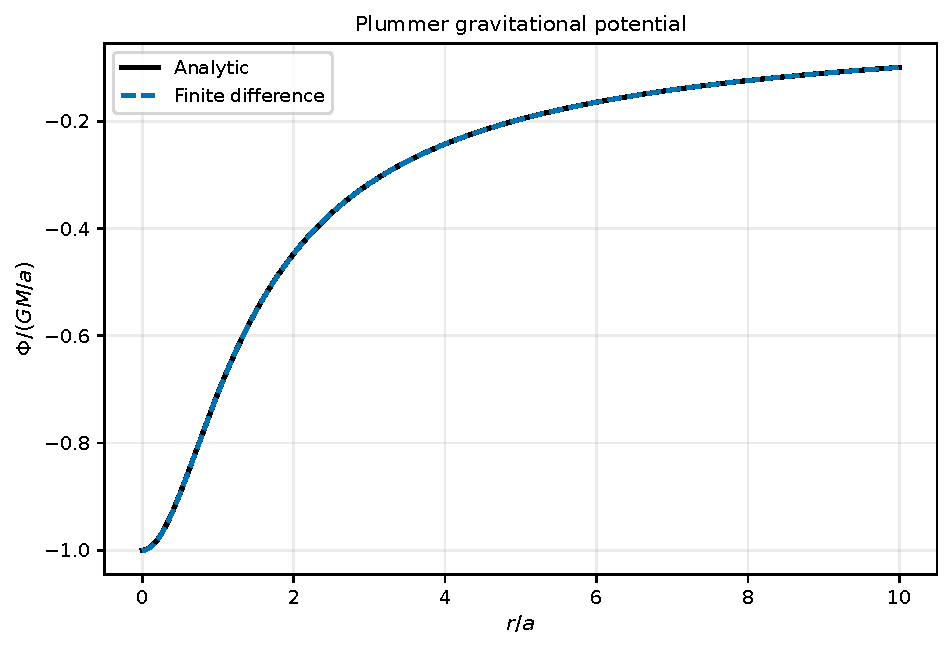
\includegraphics[width=0.68\linewidth]{ch02_potential.pdf}
\caption{Plummer ポテンシャルの有限差分解と解析解。}
\label{fig:ch2-potential}
\end{figure}

一方、差を拡大した図\ref{fig:ch2-potential-error}では、
有限差分による離散化誤差が確認できる。
今回の $N=200$ では、ポテンシャルの最大絶対誤差は
\begin{equation}
 \max_{0\le i\le N}|\Phi_{\rm num}(r_i)-\Phi_{\rm exact}(r_i)|
 =\chtwoPhiErrNTwoHundred\,\frac{GM}{a}
\label{eq:ch2-main-potential-error}
\end{equation}
である。
同じ計算を $G=M=a=1$ の無次元単位で行ったとき、連立一次方程式の最大残差は
$\max_i |(A\boldsymbol{u}-\boldsymbol{b})_i|\simeq3.85\times10^{-16}$ である。
残差の大きさは方程式の規格化に依存するが、今回用いた形では、左右のずれは浮動小数点演算の精度に近い大きさまで小さくなっている。
つまり、数値解は離散方程式 $A\boldsymbol{u}=\boldsymbol{b}$ を高い精度で満たしている。
それにもかかわらず解析解との差が残るのは、
$A\boldsymbol{u}=\boldsymbol{b}$ が Poisson 方程式そのものではなく、
二階微分を中心差分で近似して得られた離散方程式だからである。
このため、連立一次方程式を高い精度で解いても、
元の連続な Poisson 方程式に対する離散化誤差は残る。

\begin{figure}[!htbp]
\centering
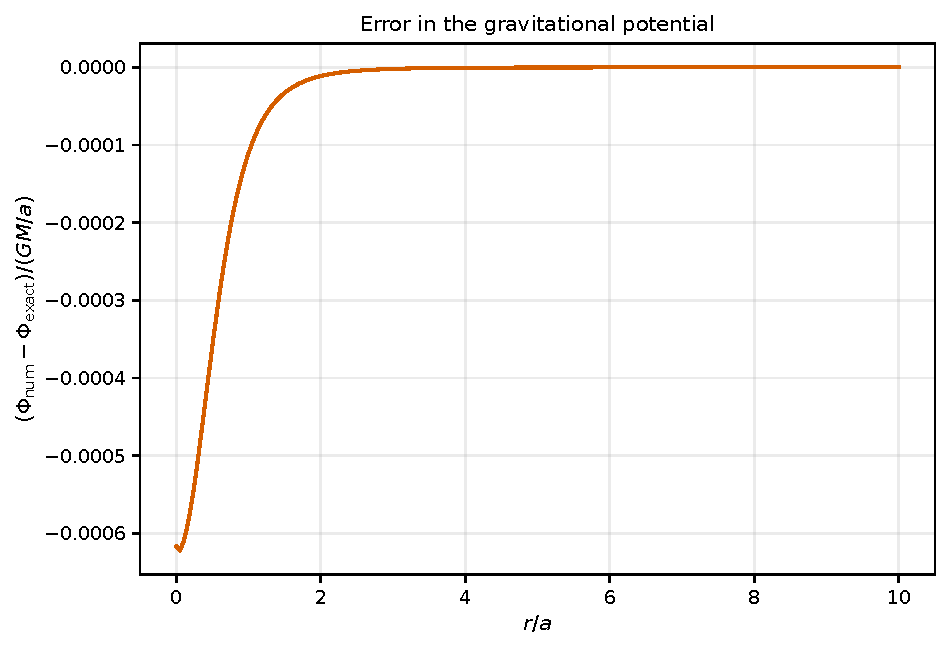
\includegraphics[width=0.68\linewidth]{ch02_potential_error.pdf}
\caption{有限差分で得た Plummer ポテンシャルの誤差。縦軸は符号付きの差 $(\Phi_{\rm num}-\Phi_{\rm exact})/(GM/a)$ であり、絶対値ではない。外側境界には解析解を与えている。}
\label{fig:ch2-potential-error}
\end{figure}


% =====================================================================
\section{Poisson 方程式の格子収束}
\label{sec:ch2-poisson-convergence}

前節では、$N=200$ の一つの格子について数値ポテンシャルを解析解と比較し、
有限差分による離散化誤差が残ることを確認した。
しかし、一つの格子で誤差を測るだけでは、
格子を細かくしたときに数値解がどのように解析解へ近づくかは分からない。
そこで本節では、格子幅 $\Delta r$ を変えて同じ計算を繰り返し、
ポテンシャルの誤差がどのように減少するかを調べる。
二階中心差分そのものの近似誤差は $O((\Delta r)^2)$ なので、
ポテンシャル全体の誤差についても2次収束が得られるかを
格子収束試験によって確認する。

計算領域は $r_{\max}=10a$ に固定し、
外側境界には前節と同じく解析値を与える。
そのうえで区間数を
\begin{equation}
 N=50,100,200,400,800
\label{eq:ch2-poisson-grids}
\end{equation}
と変化させる。
各格子では、ポテンシャルの最大絶対誤差を $GM/a$ で無次元化し、
\begin{equation}
 \epsilon_\Phi
 \equiv
 \max_{0\le i\le N}
 \frac{|\Phi_{\rm num}(r_i)-\Phi_{\rm exact}(r_i)|}{GM/a}
\label{eq:ch2-phi-error-def}
\end{equation}
として評価する。

\begin{notebookblock}{2｜Poisson 方程式の格子収束}
Notebook では5種類の格子で $\epsilon_\Phi$ を測り、両対数直線の傾きから収束次数を求める。

{\sffamily\small\color{graytext}対応セル（計算部分）}
\begin{Verbatim}[xleftmargin=2mm,fontsize=\small,frame=single,framesep=1.8mm,framerule=0.35pt,rulecolor=\color{listingframe},fillcolor=\color{listingbg}]
# 1つの格子でポテンシャルの最大誤差を測る
def poisson_error(N):
    r, _, _, phi_num, _, _ = solve_spherical_poisson_plummer(
        N=N, r_max=10.0 * a, G=G, M=M, a=a
    )
    phi_exact = phi_plummer_exact(r, G, M, a)
    dr = r[1] - r[0]
    err = np.max(np.abs(phi_num - phi_exact)) / (G * M / a)
    return dr, err

# 区間数を増やし、格子幅と誤差を記録する
N_values = np.array([50, 100, 200, 400, 800])
dr_values = []
phi_errors = []

for N_i in N_values:
    dr_i, err_i = poisson_error(int(N_i))
    dr_values.append(dr_i)
    phi_errors.append(err_i)

dr_values = np.array(dr_values)
phi_errors = np.array(phi_errors)

# log(error)-log(dr) の傾きが収束次数 p
order_phi = np.polyfit(
    np.log(dr_values), np.log(phi_errors), 1
)[0]
\end{Verbatim}
\end{notebookblock}

\begin{figure}[!htbp]
\centering
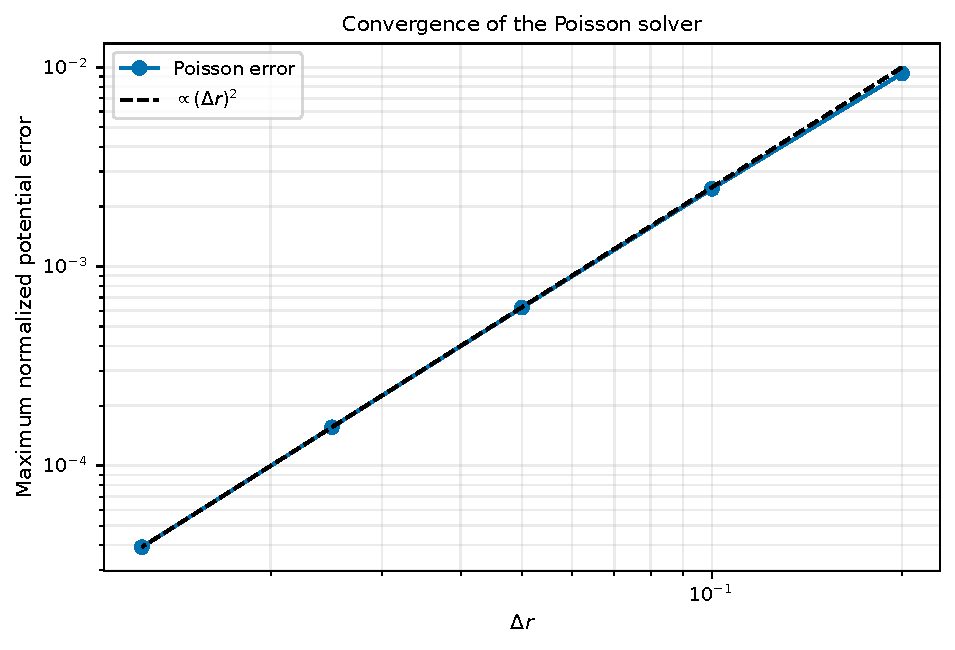
\includegraphics[width=0.68\linewidth]{ch02_poisson_convergence.pdf}
\caption{Poisson 方程式ソルバーの格子収束。破線は $\epsilon_\Phi\propto(\Delta r)^2$ を示す。}
\label{fig:ch2-poisson-convergence}
\end{figure}

5つの格子で得た誤差を両対数上で直線近似すると、$p=\chtwoPoissonOrder$ を得る。
$p$ はほぼ2であるため、ポテンシャルの数値解は格子幅 $\Delta r$ に対して2次精度で収束していることが分かる
（図\ref{fig:ch2-poisson-convergence}）。
すなわち、格子幅を半分にすると、誤差はおよそ $1/4$ に減少する。


% =====================================================================
\section{数値微分による重力加速度}
\label{sec:ch2-numerical-diff}

Poisson 方程式から $\Phi(r)$ が得られたら
\begin{equation}
 g_r(r)=-\frac{d\Phi}{dr}
\label{eq:ch2-g-from-phi}
\end{equation}
を数値微分で計算する。
ポテンシャルが格子上の値として与えられる場合には、差分して重力加速度を求める方法がある\cite{matsumoto}。
本節では、この計算を題材に数値微分の基本を学ぶ。
以下では前進差分（forward difference）、後退差分（backward difference）、中心差分（central difference）を Taylor 展開から導く\footnote{
ここでは3つの差分公式を紹介するが、内部の格子点では、同じく2点の値だけで2次精度が得られる中心差分を使うのが基本である。
前進・後退差分が必要になるのは、片側にしか格子点がない計算領域の端と、
時間方向のように一方向の値しか使えない場合である。後者の例が第3章の Euler 法である。
端点でも2次精度を保ちたい場合は、片側の3点を使う公式
$f'_0\simeq(-3f_0+4f_1-f_2)/(2\Delta r)$ がよく使われる。
ただし、流体の移流のように、流れの向きに応じて片側差分を選ばないと計算が不安定になる問題もあり、
中心差分が常に適しているわけではない。詳しくは藤井・立川\cite{fujii2020}、松本ほか\cite{matsumoto}を参照すること。}\cite{kouya2021}。
以下の $\Phi_i$ は、滑らかなポテンシャルを格子点 $r_i$ で評価した値を表す。まず差分公式自体の近似誤差を調べる。

\subsection{前進差分（forward difference）}

$r_i$ のまわりで
\begin{equation}
 \Phi_{i+1}
 =\Phi_i+\Delta r\,\Phi_i'
 +\frac{(\Delta r)^2}{2}\Phi_i''
 +\frac{(\Delta r)^3}{6}\Phi_i'''
 +O((\Delta r)^4)
\end{equation}
なので
\begin{equation}
 \boxed{
 \Phi_i'
 \simeq
 \frac{\Phi_{i+1}-\Phi_i}{\Delta r}
 }
\label{eq:ch2-forward-diff}
\end{equation}
である。
差分商から厳密な微分値 $\Phi_i'$ を引いた差の主要項は $+(\Delta r/2)\Phi_i''$ である。この誤差は $\Delta r$ に比例するので1次精度である。
重力加速度に使うと Listing 2.2 のようになる。

\begin{listingbox}{2.2　前進差分}
\begin{Verbatim}[fontsize=\small]
def gravity_forward(r, phi):
    dr = r[1] - r[0]
    return r[:-1], -(phi[1:] - phi[:-1]) / dr
\end{Verbatim}
\end{listingbox}

返す半径が \texttt{r[:-1]} なのは、差分商 $(\Phi_{i+1}-\Phi_i)/\Delta r$ を $r_i$ での微分の近似とするためである。

\subsection{後退差分（backward difference）}

同様に
\begin{equation}
 \Phi_{i-1}
 =\Phi_i-\Delta r\,\Phi_i'
 +\frac{(\Delta r)^2}{2}\Phi_i''
 -\frac{(\Delta r)^3}{6}\Phi_i'''
 +O((\Delta r)^4)
\end{equation}
より
\begin{equation}
 \boxed{
 \Phi_i'
 \simeq
 \frac{\Phi_i-\Phi_{i-1}}{\Delta r}
 }
\label{eq:ch2-backward-diff}
\end{equation}
である。
差分商から厳密な微分値を引いた差の主要項は $-(\Delta r/2)\Phi_i''$ であり、やはり1次精度である。

\begin{listingbox}{2.3　後退差分}
\begin{Verbatim}[fontsize=\small]
def gravity_backward(r, phi):
    dr = r[1] - r[0]
    return r[1:], -(phi[1:] - phi[:-1]) / dr
\end{Verbatim}
\end{listingbox}

前進差分と後退差分のコードは同じ2点差を計算している。
違いは、その差をどの格子点の微分とみなすかである。
後退差分では \texttt{r[1:]} を返す。

\subsection{中心差分（central difference）}

前進側と後退側の Taylor 展開を4次の項まで含めて引き算すると、偶数次の項が消えて
\begin{equation}
 \Phi_{i+1}-\Phi_{i-1}
 =2\Delta r\,\Phi_i'
 +\frac{(\Delta r)^3}{3}\Phi_i'''
 +O((\Delta r)^5)
\end{equation}
である。
したがって
\begin{equation}
 \boxed{
 \Phi_i'
 \simeq
 \frac{\Phi_{i+1}-\Phi_{i-1}}{2\Delta r}
 }
\label{eq:ch2-central-diff}
\end{equation}
を得る。
差分商から厳密な微分値を引いた差の主要項は
$(\Delta r)^2\Phi_i'''/6$ なので、
中心差分の誤差は $O((\Delta r)^2)$ であり、2次精度である。
これは、同じ点で評価した前進差分と後退差分を平均すると、主要な1次誤差が互いに相殺されることに対応している。

\begin{listingbox}{2.4　中心差分}
\begin{Verbatim}[fontsize=\small]
def gravity_central(r, phi):
    dr = r[1] - r[0]
    return r[1:-1], -(phi[2:] - phi[:-2]) / (2.0 * dr)
\end{Verbatim}
\end{listingbox}

この3点中心差分は左右の格子点を必要とするため、計算領域の両端にはそのまま適用できない。
したがって、この関数が返す半径配列は \texttt{r[1:-1]} である。

\subsection{Plummer 球への適用}

以上の3つの差分公式を、Plummer 球のポテンシャルに適用する。
Poisson 方程式の数値解 $\Phi_{\rm num}$ を微分すると、ポテンシャルに含まれる離散化誤差と数値微分そのものの誤差が重力加速度に同時に含まれる。
そこで、差分公式そのものの性質を調べるため、解析ポテンシャル $\Phi_{\rm exact}$ を格子点で評価して用いる。

$N=200$、$r_{\max}=10a$ の格子上で、同じ解析ポテンシャルに前進差分・後退差分・中心差分を適用する。
各関数が返す半径配列は差分公式によって異なるため、それぞれの評価位置における解析解と比較する。

\begin{notebookblock}{2｜数値微分による重力加速度}
同じ格子上で評価した解析ポテンシャルに、
前進差分・後退差分・中心差分を適用する。

{\sffamily\small\color{graytext}対応セル（計算部分）}
\begin{Verbatim}[xleftmargin=2mm,fontsize=\small,frame=single,framesep=1.8mm,framerule=0.35pt,rulecolor=\color{listingframe},fillcolor=\color{listingbg}]
# 一つの格子で解析ポテンシャルを評価する
N = 200
r_max = 10.0 * a
r_diff = np.linspace(0.0, r_max, N + 1)
phi_for_diff = phi_plummer_exact(r_diff, G, M, a)

# 3つの差分公式で重力加速度を求める
r_f, g_forward = gravity_forward(r_diff, phi_for_diff)
r_b, g_backward = gravity_backward(r_diff, phi_for_diff)
r_c, g_central = gravity_central(r_diff, phi_for_diff)
\end{Verbatim}
\end{notebookblock}

図\ref{fig:ch2-differentiation}に、この計算で得られた重力加速度を解析解とともに示す。
この格子では、3つの差分公式はいずれも解析解に近い値を与える。

\begin{figure}[!htbp]
\centering
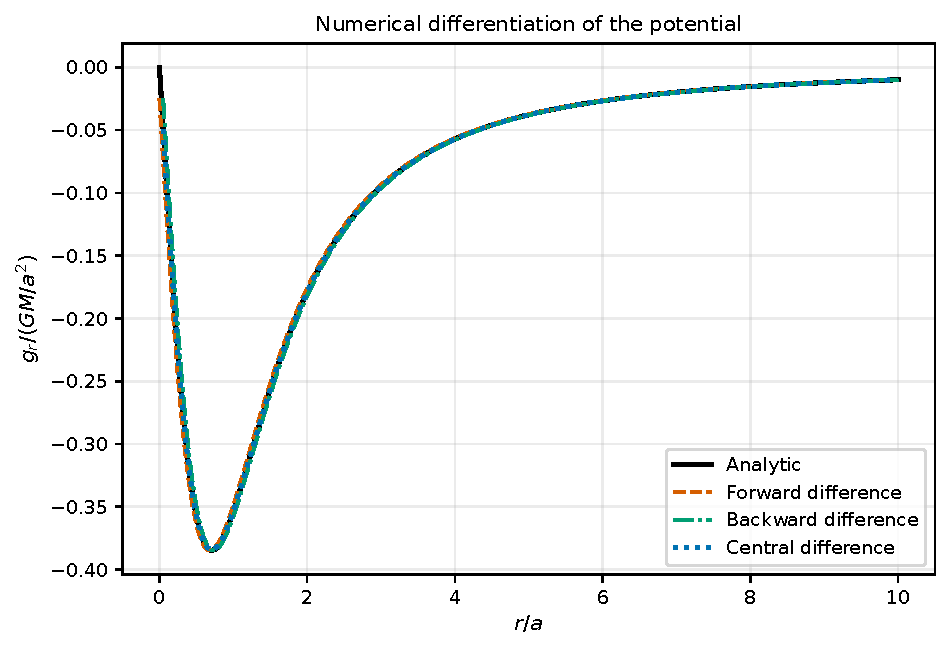
\includegraphics[width=0.68\linewidth]{ch02_differentiation.pdf}
\caption{$N=200$、$r_{\max}=10a$ の格子上で、解析的な Plummer ポテンシャルを前進・後退・中心差分して得た重力加速度。}
\label{fig:ch2-differentiation}
\end{figure}

一つの格子で結果を比較するだけでは、格子を細かくしたときに誤差がどの速さで減少するかは分からない。
この点を次節の格子収束試験で調べる。

% =====================================================================

\section{前進・後退・中心差分の収束比較}
\label{sec:ch2-diff-convergence}

前節では、一つの格子上で解析ポテンシャルを数値微分し、3つの差分公式から得られる重力加速度を比較した。
本節では格子幅を変えて同じ計算を繰り返し、前進差分・後退差分の1次収束と中心差分の2次収束を数値的に確認する。

数値微分そのものの収束性を調べるため、前節と同じく解析ポテンシャル $\Phi_{\rm exact}$ を入力として用いる。
計算領域を $r_{\max}=10a$ に固定し、区間数を
\begin{equation}
 N=50,100,200,400,800
\end{equation}
と変えて、5種類の格子で誤差を測る。

格子を変えると、各差分公式が重力加速度を返す格子点の位置も変わる。
そこで、すべての格子で同じ物理的な半径範囲を比較するため、
\begin{equation}
 0.2a\le r\le5a
\label{eq:ch2-diff-range}
\end{equation}
に含まれる評価点だけを用いる。
各差分公式について、規格化した最大絶対誤差を
\begin{equation}
 \epsilon_{g,\mathrm{fixed}}
 \equiv
 \max_{\substack{i\\0.2a\le r_i\le5a}}
 \frac{|g_{r,\mathrm{num}}(r_i)-g_{r,\mathrm{exact}}(r_i)|}{GM/a^2}
\label{eq:ch2-gravity-error-fixed}
\end{equation}
と定義する。
ここで $g_{r,\mathrm{num}}$ は各差分公式から得た重力加速度である。
分母の $GM/a^2$ は一定の基準量なので、
$\epsilon_{g,\mathrm{fixed}}$ は規格化した絶対誤差であり、
各点での相対誤差ではない。

\begin{notebookblock}{2｜数値微分の格子収束}
各格子について、解析ポテンシャルを3つの差分公式で微分し、
式\eqref{eq:ch2-gravity-error-fixed}の最大誤差を測る。
この処理を補助関数 \texttt{differentiation\_errors} にまとめる。

{\sffamily\small\color{graytext}対応セル（補助関数）}
\begin{Verbatim}[xleftmargin=2mm,fontsize=\small,frame=single,framesep=1.8mm,framerule=0.35pt,rulecolor=\color{listingframe},fillcolor=\color{listingbg}]
def differentiation_errors(N):
    r_max = 10.0 * a
    r = np.linspace(0.0, r_max, N + 1)
    dr = r[1] - r[0]
    phi = phi_plummer_exact(r, G, M, a)

    r_f, g_f = gravity_forward(r, phi)
    r_b, g_b = gravity_backward(r, phi)
    r_c, g_c = gravity_central(r, phi)

    def max_error(r_eval, g_num):
        mask = (r_eval >= 0.2 * a) & (r_eval <= 5.0 * a)
        g_exact = gravity_plummer_exact(r_eval, G, M, a)
        return np.max(np.abs(g_num[mask] - g_exact[mask])) / (G * M / a**2)

    return dr, max_error(r_f, g_f), max_error(r_b, g_b), max_error(r_c, g_c)
\end{Verbatim}

{\sffamily\small\color{graytext}対応セル（収束次数の測定）}
\begin{Verbatim}[xleftmargin=2mm,fontsize=\small,frame=single,framesep=1.8mm,framerule=0.35pt,rulecolor=\color{listingframe},fillcolor=\color{listingbg}]
# 5種類の格子で3手法の最大誤差を測る
N_diff = np.array([50, 100, 200, 400, 800])
results = np.array([differentiation_errors(int(N_i)) for N_i in N_diff])

dr_diff = results[:, 0]
err_forward = results[:, 1]
err_backward = results[:, 2]
err_central = results[:, 3]

# log(error)-log(dr) の傾きから収束次数を求める
order_forward = np.polyfit(np.log(dr_diff), np.log(err_forward), 1)[0]
order_backward = np.polyfit(np.log(dr_diff), np.log(err_backward), 1)[0]
order_central = np.polyfit(np.log(dr_diff), np.log(err_central), 1)[0]
\end{Verbatim}
\end{notebookblock}

5つの格子で得た誤差を両対数上で直線近似すると、
\begin{equation}
 p_{\rm f}=\chtwoForwardOrder,
 \qquad
 p_{\rm b}=\chtwoBackwardOrder,
 \qquad
 p_{\rm c}=\chtwoCentralOrder
\label{eq:ch2-diff-orders}
\end{equation}
を得る。添字 $\mathrm f,\mathrm b,\mathrm c$ は、それぞれ前進・後退・中心差分を表す。
図\ref{fig:ch2-differentiation-convergence}に示すように、
前進差分と後退差分はほぼ1次精度、中心差分はほぼ2次精度で収束しており、
前節で求めた各差分公式の誤差評価と一致する。
前進差分と後退差分の測定値が厳密に1にならないのは、
有限の格子幅では主要な1次誤差だけでなく、より高次の誤差項も寄与するためである。
格子をさらに細かくすると、それらの影響は小さくなり、
測定される収束次数は1に近づく。

\begin{figure}[!htbp]
\centering
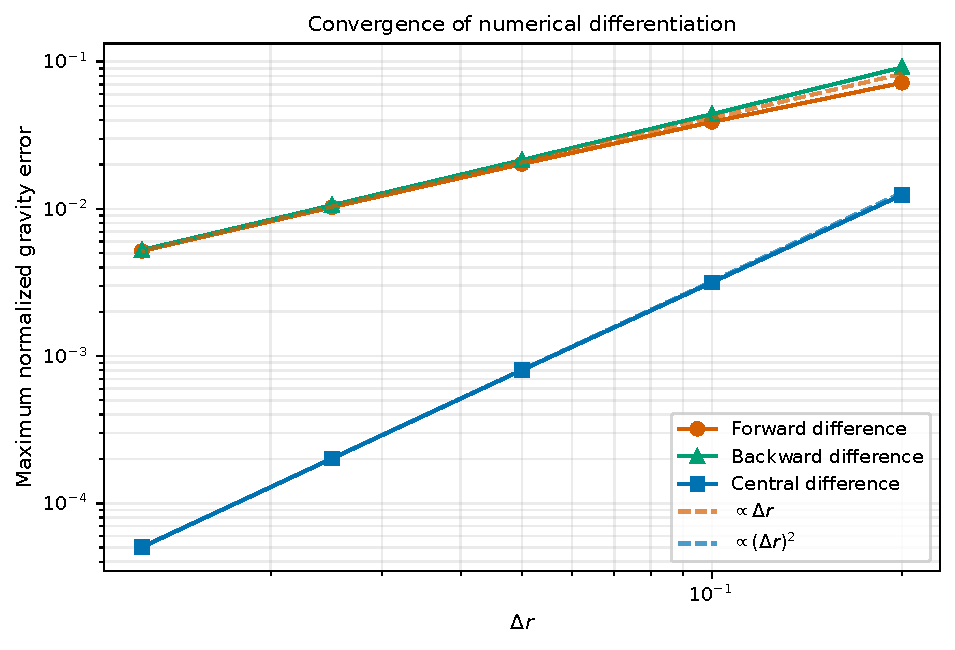
\includegraphics[width=0.68\linewidth]{ch02_differentiation_convergence.pdf}
\caption{解析的な Plummer ポテンシャルを数値微分したときの格子収束。$0.2a\le r\le5a$ で測った規格化最大絶対誤差を示す。前進・後退差分はほぼ1次、中心差分はほぼ2次で収束する。}
\label{fig:ch2-differentiation-convergence}
\end{figure}


以上で、密度分布から Poisson 方程式を解いてポテンシャルを求め、
その数値微分から重力加速度を計算するための手順がそろった。
ここまでの収束試験では、Poisson 方程式の求解と数値微分を分けて検証した。
Notebook 2 の総合演習では、数値ポテンシャル $\Phi_{\rm num}$ を中心差分して
重力加速度を求め、解析解および第1章の累積台形則による内包質量から得た結果と比較する。

% =====================================================================
\begin{topicblock}{偏微分方程式の型と境界条件}
本章で扱った Poisson 方程式は、\textbf{楕円型（elliptic）}偏微分方程式の代表例である。
この境界値問題では、内部の方程式と境界条件を合わせ、領域全体で互いに結合した未知数を求める。
本章では中心と外側に条件を与え、有限差分で得た連立一次方程式を解いた。
付録\ref{app:linear-systems}の反復法を使う場合も、領域全体の方程式を満たす解へ近づける点は同じである。

熱伝導や拡散を記述する\textbf{放物型（parabolic）}と、波や移流を記述する\textbf{双曲型（hyperbolic）}の方程式も、宇宙流体計算で現れる。
有限領域でこれらの時間発展を求める問題は、初期条件と境界条件を組み合わせた\textbf{初期境界値問題（initial-boundary value problem）}として扱う。
正の拡散係数を持つ拡散方程式では、初期分布に加え、空間領域の境界全体で各時刻の条件を定める。
一方、双曲型では情報が有限の速さで伝わる経路を\textbf{特性曲線}と呼び、境界で与える独立な条件の数は、領域へ流入する特性の数で決まる。
例えば一定方向に進む移流では、流入側に値を与え、流出側の値は内部から伝わる解によって決まる。
この場合、流出側に独立な値を追加して固定してはいけない。
ただし、流出境界近くの数値更新に必要な値を、内部から外側へ延長する処理は必要になり得る。

本章では既知の境界値を右辺へ移したが、別の実装方法として、計算領域の外側に仮想的な値を置き、境界近傍でも内部と同じ形の更新式を使う方法がある。
格子法の流体計算で用いる\textbf{ゴーストセル（ghost cell）}はこの考え方に対応し、付録\ref{app:axisym-poisson}の対称軸の仮想点とも共通する。
例えば、周期境界では反対側の値をコピーし、反射境界では境界をはさんで対称な位置の値をコピーして、境界に垂直な速度成分の符号を反転する。
流出境界では内部の値を外挿する方法があるが、すべての波を無反射で通す保証はない。
必要な物理的条件と、その条件を実装する処理を分けて考えることが重要である。
境界条件とゴーストセルの扱いは、藤井・立川\cite{fujii2020}、松本ほか\cite{matsumoto}を参照すること。
\end{topicblock}

\begin{topicblock}{時間発展問題の時間積分と連立一次方程式}
時間発展を含む偏微分方程式でも、空間方向を有限差分などで離散化すると、各格子点の値についての連立常微分方程式が得られる。
これを時間方向へ進める方法には、陽的な方法と陰的な方法がある。

既知の状態と、すでに計算した途中の状態から、順に更新量を求める方法を\textbf{陽的な時間積分（explicit time integration）}という。
第3章で扱う Euler 法と陽的 Runge--Kutta 法では、時間更新の未知量について連立方程式を解く必要はない。
一方、空間離散化と組み合わせた時間刻みの制約を満たす必要がある。
例えば、一次元の圧縮性流体で全セルに共通の時間刻みを使う場合には、
\[
 \Delta t\le C_{\rm CFL}\min_i\frac{\Delta x_i}{|v_i|+c_{{\rm s},i}}
\]
という\textbf{CFL 条件（Courant--Friedrichs--Lewy condition）}が重要になる。
$\Delta x_i$ はセル幅、$v_i$ は流速、$c_{{\rm s},i}$ は音速であり、最も厳しいセルの条件を使う。
$C_{\rm CFL}$ の許容値は数値手法に依存し、この条件を満たすだけで任意の空間離散化が安定になるわけではない。
一定の拡散係数を持つ拡散方程式の陽解法では、許される時間刻みの上限は典型的に $\Delta t_{\max}\propto(\Delta x)^2$ となる。
高次精度の公式を選ぶことと、安定に時間発展を計算することは別である。

次の時刻や計算途中の未知の値を含む式を立て、その式を解いて更新する方法を\textbf{陰的な時間積分（implicit time integration）}という。
線形な問題では連立一次方程式に帰着するが、非線形な問題では非線形方程式を解く必要がある。
例として、本章の $u=r\Phi$ とは区別して拡散する量を $w(x,t)$ と書き、一定の拡散係数 $D>0$ を持つ方程式
\[
 \frac{\partial w}{\partial t}=D\frac{\partial^2 w}{\partial x^2}
\]
を考える。
一様格子上の値を $w_i^n\simeq w(x_i,t_n)$ とし、二階微分を中心差分、時間方向を後退 Euler 法で離散化すると、
\[
 \frac{w_i^{n+1}-w_i^n}{\Delta t}
 =D\frac{w_{i+1}^{n+1}-2w_i^{n+1}+w_{i-1}^{n+1}}{(\Delta x)^2}
\]
である。
これを整理すると、
\[
 -\alpha w_{i-1}^{n+1}+(1+2\alpha)w_i^{n+1}-\alpha w_{i+1}^{n+1}=w_i^n,
 \qquad \alpha=\frac{D\Delta t}{(\Delta x)^2}
\]
となる。
境界値を指定すれば、本章と同じ三重対角構造の連立一次方程式を各ステップで解くことになる。
この線形拡散問題に対する後退 Euler 法では、陽解法の拡散安定条件を避けられるが、大きな時間刻みでも時間変化を正確に追えるという意味ではない。
安定性による制約と、精度のために必要な時間刻みを区別する。

宇宙流体計算では、流体部分を陽的に進め、熱伝導や輻射の拡散など、時間刻みの制約が厳しい過程を陰的に扱うことがある。
また、流体の時間更新が陽的でも、自己重力を求めるには Poisson 方程式を解く。
本章では密度を固定したが、自己重力流体では密度分布が変わるため、時間積分の各段階と整合する密度から重力場を更新する必要がある。
詳しい解法は藤井・立川\cite{fujii2020}、松本ほか\cite{matsumoto}、自己重力との組合せは富阪ほか編\cite{tomisaka2007}を参照すること。
\end{topicblock}

